
In this section, we present the high-level architecture of our CONFINE framework. We consider the main functionalities of each component, avoiding details on the employed technologies discussed in the next sections. After introducing the architecture, we focus on the \Compo{Secure Miner}, a core component of our contribution.

\subsection{CONFINE architecture at large}
Our architecture involves different organizational ecosystems characterized by one or more machines. An organization may take at least one of the following roles: 
\begin{inparadesc}
\item[provisioning] if it delivers local event logs to be collaboratively mined;
\item[mining] if it applies process mining algorithms using event logs retrieved from provisioners.
\end{inparadesc}
% Provisioners collaborate to achieve common objectives and compose inter-organizational business processes whose event logs are scattered across multiple places. 
% Provisioners produce event logs, recording the operations executed to complete their part in the inter-organizational business process.
In \cref{fig:architecture_diagram}, we propose the high-level schematization of our solution.
In our solution, every organization hosts one or more \Compo{Node}s. Depending on the played role, \Compo{Node}s come endowed with a \Compo{Provisioner} or a \Compo{Secure Miner} component, or both. The \Compo{Provisioner} component consists of the following two main sub-components. The \begin{inparadesc}
\item[\Compo{Log Recorder}] registers the events taking place in the organizations' systems. The
\item[\Compo{Log Provider}] delivers on-demand data to mining players.
\end{inparadesc}
The \Actor{Hospital} (as well the other parties in our running example) records Alice and Bob's traces using the \Compo{Log Recorder}. The \Compo{Log Recorder} is queried by the \Compo{Log Provider} for event logs to be made available for mining. The latter controls access to local event logs by authenticating data requests by miners and rejecting those that come from unauthorized parties.
In our motivating scenario, the \Actor{Specialized clinic}, \Actor{Pharmaceutical company}, and the \Actor{Hospital} leverage \Compo{Log Provider}s to authenticate the miner party before sending their logs.  The \Compo{Secure Miner} component
% \Compo{Log Provider}s reject demands from unauthorized parties and only permit \texttt{Secure Miners} to use the data. 
% The \Compo{Secure Miner} 
shelters external event logs inside a protected environment to preserve data confidentiality and integrity.
Notice that \Compo{Log Provider}s accept requests issued solely by \Compo{Secure Miner}s. 
Next, we provide an in-depth focus on the latter.
% We provide an in-depth focus on this key component in the following.
\begin{comment}
\begin{figure}[t]
	\centering
	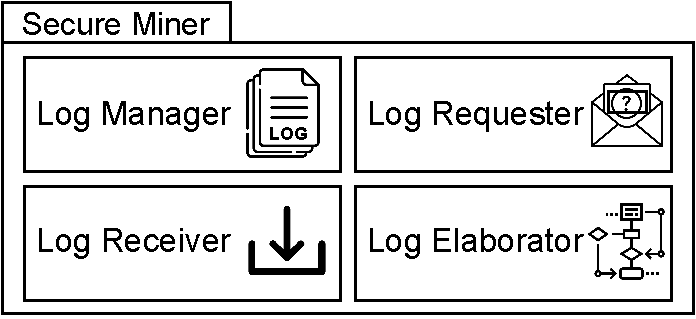
\includegraphics[width=0.5\linewidth]{content/figures/secureminersad.pdf}
	\caption{Subcomponents of the Secure Miner.}
	\label{fig:trusted_miner}
\end{figure}
\end{comment}

\begin{figure}[t]
	\centering
	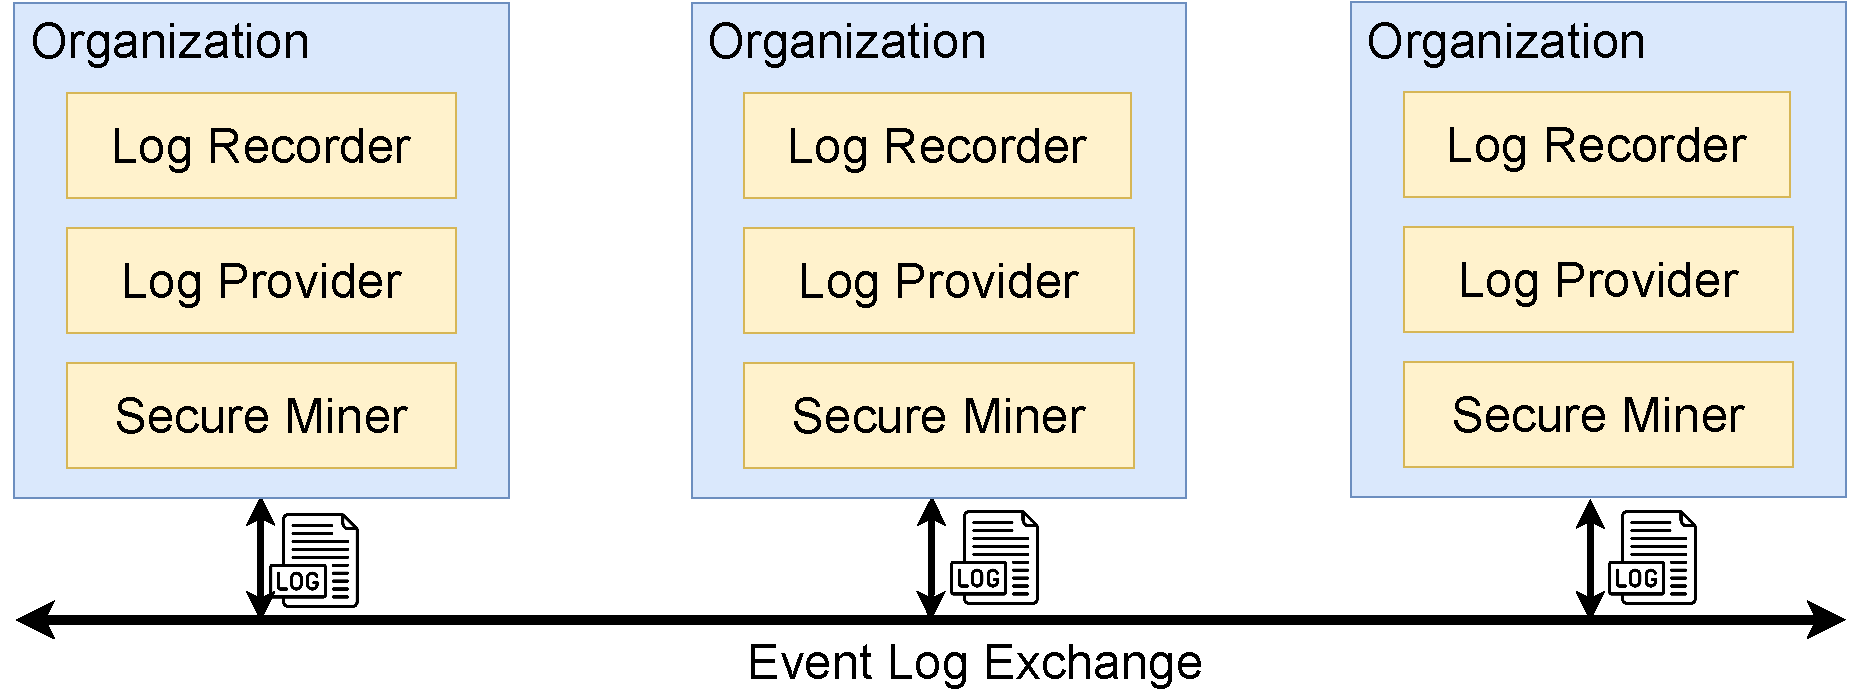
\includegraphics[width=0.79\linewidth]{content/figures/architecturediagram.pdf}
	\caption{High-level architectural overview.}
	\label{fig:architecture_diagram}
\end{figure}

\begin{wrapfigure}[9]{r}{0.4\textwidth}
	\vspace{-2em}
	\centering
	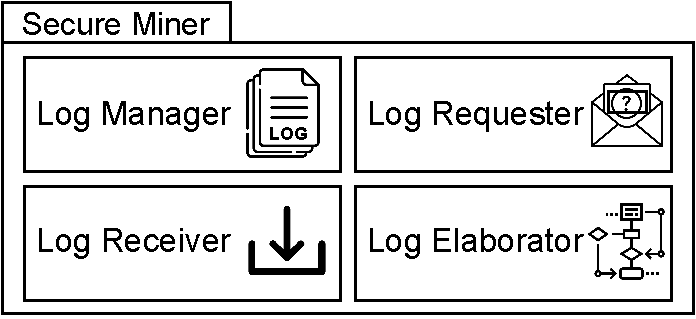
\includegraphics[width=1\textwidth]{content/figures/secureminersad.pdf}
	\caption[A gull]{Sub-components of the \\Secure Miner.}
	\label{fig:trusted_miner}
	\vspace{-6pt}
\end{wrapfigure} 
\subsection{Secure Miner}
The primary objective of the \Compo{Secure Miner} is to allow miners to securely execute process mining algorithms using event logs retrieved from provisioners such as the \Actor{Specialized clinic}, \Actor{Pharmaceutical company}, and the \Actor{Hospital} of our running example. \Compo{Secure Miner}s are isolated components that guarantee data inalterability and confidentiality. In \cref{fig:trusted_miner}, we show a schematization of the \Compo{Secure Miner}, which consists of four sub-components:
\begin{inparaenum}[\itshape(i)\upshape]
    \item The \Compo{Log Requester};
    \item The \Compo{Log Receiver};
    \item The \Compo{Log Manager}; 
    \item The \Compo{Log Elaborator}.
\end{inparaenum}
%Event logs belonging to provisioners are locked in the \Compo{Secure Miner}.
%We handle  data via the 
The \Compo{Log Requester} and the \Compo{Log Receiver} are the sub-components that we employ during the event log retrieval. \Compo{Log Requester}s send authenticable data requests to the \Compo{Log Provider} component of provisioners. The \Compo{Log Receiver} collects event logs sent by \texttt{Log Providers} and entrusts them to the \Compo{Log Manager}, securing them from accesses that are external to the \Compo{Secure Miner}.
Miners of our motivating scenario, such as the \Actor{University} and the \Actor{National Institute of Statistics}, employ these three components to retrieve and store Alice and Bob's data. The \Compo{Log Elaborator} merges the event data locked in the \Compo{Secure Miner} to have a global view of the inter-organizational process comprehensive of activities executed by each involved party. Thereupon, it executes process mining algorithms in a protected environment, inaccessible from the outside computation environment.
In our motivating scenario, the \Compo{Log Elaborator} combines the traces of Alice (i.e., $T^H_{312}$, $T^S_{312}$, and $T^C_{312}$) and Bob (i.e, $T^H_{711}$, $T^S_{711}$, and $T^C_{711}$), generates the chronologically sorted traces $T_{312}$ and $T_{711}$, and feeds them into the mining algorithms (see the bottom-right quadrant of \cref{tab:trace}).



